\documentclass{article}


\usepackage[T1]{fontenc}
\usepackage{mathptmx}
\usepackage{graphicx} % Required for inserting images
\usepackage{hyperref}
\usepackage{tocloft}



\title{\Huge A guide for fellow PhDs}
\author{Emanuele D'Allestro}
\date{\Large July 2025\\[1cm] \normalsize © 2025 Emanuele D'Allestro. All rights reserved.}
\begin{document}

\maketitle
\newpage
\tableofcontents

\newpage

\section{Working environment \& Employment}
\textit{This section has been developed with information from SULF association.}

\subsection{Admission to PhD studies and contracts}
In Sweden, all doctoral candidates are admitted as students to a PhD program,
and the vast majority are employed by their university as doctoral candidates. This means that you are both a student
and an employee. While there is no limit on how long you can remain a student
in a PhD program, your employment as a doctoral candidate is capped at a
maximum of four years with full-time
studies. However, your employment can be extended indefinitely due to
factors like parental leave or illness.
For PhD programs involving additional
departmental duties (such as teaching), the maximum employment period is
five years.The initial employment may
not be for longer than one year. Employment may be renewed for no more
than two years at a time. Employment
as a doctoral candidate is usually full time. However, you can choose to be
employed at a lower rate, the minimum being 50\%. Employment as a doctoral
candidate is regulated in Chapter 5 of the Higher Education Ordinance, (Hög
skoleförordningen).

Contractual terms of employment are negotiated in the form of collective
agreements between your university and the trade unions.

\subsection{Financing}
In most cases, doctoral candidates in Sweden are employed as doctoral
candidates, meaning you receive a salary from the university. Remember
that salaries should increase in accordance with local collective agreements
(lokala kollektivavtal), and other local
policies. Check your university website for the relevant information, or contact your administration office or local trade
union representatives for details about the salary system.

Some doctoral candidates receive their
income from a scholarship. Having a
scholarship is not the same as being
employed, because these doctoral
candidates work under different rules,
with fewer protections. For example, if
you are a scholarship recipient, you do
not earn a pension and are not covered
by collective agreements.

Yet other doctoral candidates are employed by some organisation other than
the university itself. This commonly
applies in healthcare, with clinic-based
doctoral candidates often employed by the local region, or industry-based
doctoral candidates in science and engineering. In this case, your employer
has entered into an agreement with your university, in which the employer
agrees to allocate paid working time in your employment for you to pursue
your doctoral education. Salaries for clinical and industry PhDs should be
at least equal to university-employed
doctoral salaries and are often higher.
Even if you are employed by a different
organisation, you are a student at your
university, and have the same educational rights as other doctoral candidates
there. Your employment conditions, however, may be different.

\subsection{Salary review}
In order to step up in the salary review, you must hit 30, 50 or 80\% of your research objective.
In the future the review will be shifted on a time basis but for now it is different for each supervisor.
There is currently no official way to determine it, but the PhDChapter suggest to use this framework to determine your progress:

\begin{figure}[h]
    \centering
    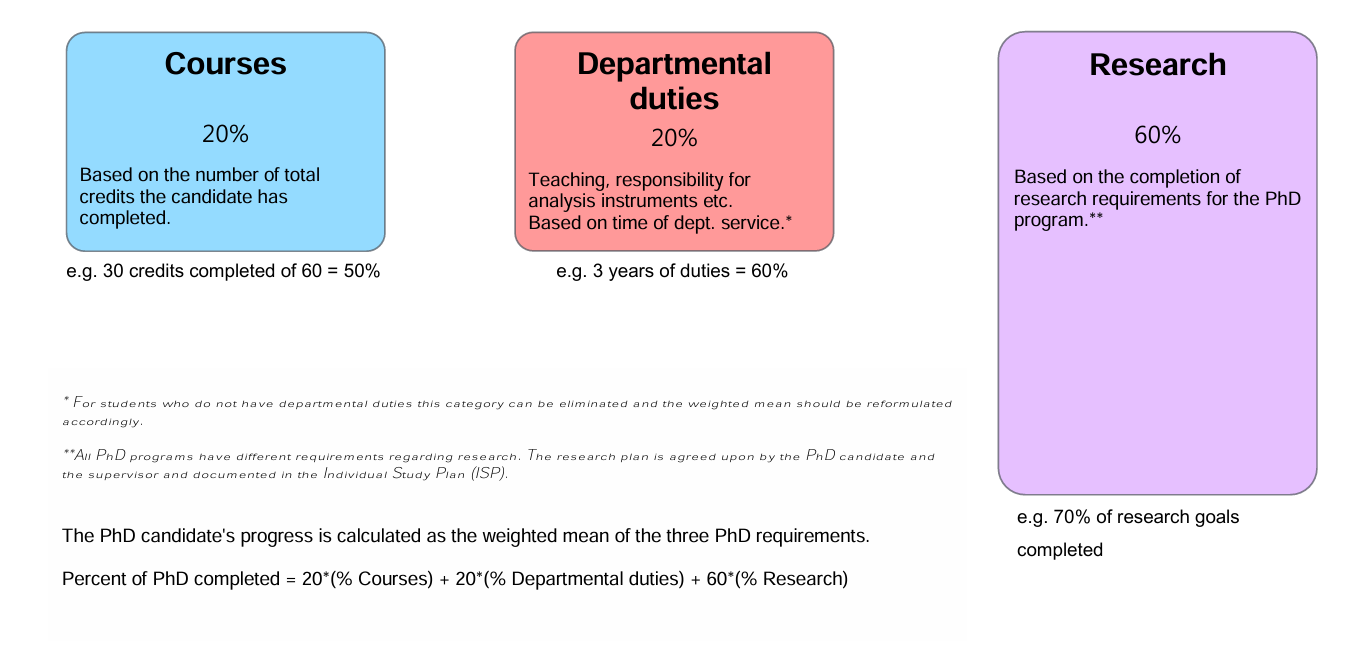
\includegraphics[width=1\linewidth]{image/progressPhd.png}
    \caption{PhD Chapter framework for tracking research progress.}
    \label{fig:progressPhD}
\end{figure}

\subsection{Duty, Research and Teaching}
Phd in Sweden is 4.6 years long as your research pace, normally, will be set at  around 84\%. The remaining 16\% usually is related to teaching duty you have to do. Usually about 2 courses (can be either bachelor or master courses) and some exams corrections.

If you are employed as a doctoral candidate, you may be required to dedicate
up to 20\% of your time to departmental work (teaching, supervision, administrative, or research tasks) in which case, your contract shall be prolonged by an equivalent amount of time, up to a maximum of five years.

\subsection{Sick leave}
It is important to report sick leave. Typically, this is done through PRIMULA or a similar HR system. As an employee, you will receive sick pay, (approximately 80\% of your salary, 90\% if on long
term sick leave), for the period that you report sick. Special rules apply to the first sick day.  If you are employed as a doctoral candidate, your contract should be extended for any days missed
due to sickness. In cases where your sick leave lasts for longer than 7 calendar days, you will need a doctor’s note. After 14 calendar days, you will need to report this to the Social Insurance
Agency, (Försäkringskassan) – the employer helps you with this. When you receive a medical certificate after 14 days, the healthcare provider sends it directly to 1177 or Försäkringskassan. As an employee, it is your responsibility to forward the sickness certificate to your employer. A representative for your employer, typically the HR person in charge at the department, will then register your sick leave with Försäkringskassan. Once the university has registered it, you will need to log into Försäkringskassan and apply to receive compensation for the sick leave days. When you apply to Försäkringskassan, you will be asked to complete forms where you provide details such as your current salary, the number of sick leave days, and whether you are paid by the hour or on a daily basis. The payment decision process at Försäkringskassan occurs in two steps: Salary Base Decision: Försäkringskassan first decides the salary base on which they will calculate your sick leave payment. You will receive a letter informing you of their decision regarding the salary base, which is usually your current salary.Sick Leave Payment Decision: In the second step, Försäkringskassan determines the actual payment based on the number of sick leave days.

Included in the membership is a health insurance that gives compensation for two months if you are sick more than three months, see folksam.se/forbund/
sulf/member-health-insurance. This insurance also covers if you are in need of preventive care or need to be at home from work to take care of a close relative or a seriously ill child. Additional
health insurance can be purchased from Folksam with membership discount.

\subsection{Parental leave}
Parental leave benefits are complex, but employed doctoral candidates have the right to access the same benefits as other employees. The Parental Leave Act entitles you to take time away from
work and stay home to provide childcare for a certain number of days, depending on specifics such as the age of the child. If you are planning to have a child or apply for parental leave, even if you
already have a child, you should contact your union, the HR department at your university and the Social Insurance Agency (Försäkringskassan), to ask about your specific case. SULF offers
a parental leave manual to members, and you can find this when you login at sulf.se/en/log-in or scan the QR code below. For a short overview, see sulf.se/en/work-salary-and-benefits/parental
leave/parental-leave-for-doctoral candidates. For more information, see  forsakringskassan.se.

\subsection{Trade unions, Rights and Legal information}
In Sweden, working conditions are regulated to a greater extent through collective agreements than by legislation. These agreements are negotiated by unions and individual employers. Therefore approximately 70\% of all Swedish employees are members of a union, and these numbers are even higher for state employees. Unions are open to all, regardless of nationality or type
of employment. Union membership can facilitate access to many kinds of assistance (e.g. information related to doctoral studies and legal assistance).

SULF, the Swedish Association of University Teachers and Researchers, is the union and professional organisation with the most members in academia. SULF is a non-politically, non-religiously affiliated union. SULF has local boards at most universities and a national office. As a member you can always receive information and support whenever you need it. We know the special regulations that apply to academia, and social insurance systems and residence permit rules for our members working at universities.

As a PhD, you are both entitled to be in the Labour Union as well as in the Student Union. You can reap the benefits from both. For Student Union, refer to THS. For labour unions, refer to SULF or many others are available. In need of legal andvices but also general help from the Union association, you can look up at SULF here: \url{https://sulf.se/en/work-salary-and-benefits/doctoral-candidate-doctoral-studies/}.

\subsection{Insurance}
As an employed doctoral candidate,
you are insured by your university for
various work-related risks, but you may
want to purchase additional forms of
insurance. A-kassas are the unemploy
ment insurance funds that normally
provide unemployment compensation
to their members who lose their jobs.
In order to be able to receive unem
ployment compensation, you need to
be a member of an a-kassa and to have
paid a small monthly fee for at least 12
months before the end of your employ
ment. You cannot receive compensa
tion from the a-kassa before you have
handed in your thesis to be printed,
even if you have run out of funding.
This is because you are regarded as an
active student in this situation and not
a job seeker.

The benefits paid out by the a-kassa
income insurance system are lower
than salaries and are supposed to co
ver about 80 percent of your previous
salary. However, there is also a ceiling
which means that you cannot get more
then 80 percent of 33 000 SEK/month
before tax no matter which salary you
have had. SULF has therefore introdu
ced a top-up income insurance, which
pays out extra money if you have a hig
her salary while you are unemployed
and receiving a-kassa benefits. When
you are a member of SULF, you are au
tomatically enrolled in this income in
surance at no additional cost. However,
keep in mind that you still need to be
enrolled with a-kassa, separately from
your SULF membership.

You should also consider purchasing
home insurance. In Sweden, “home
insurance” refers to a basic personal in
surance package that typically includes
insurance for your house, your belong
ings (also outside the house), liability
for damages to third parties, legal ex
penses and travel insurance.
SULF negotiates discounts on common
insurance products on behalf of its members. Instead, SULF has an agreement with the insurance company Folksam entailing
that SULF members can purchase insurance from Folksam at heavily discounted prices.

\section{The PhD Program (Academic)}

\subsection{General Study Plan (ASP)/Syllabus}
In line with national university guide lines, each PhD or licentiate program
must have a General Study Plan, also known as a syllabus (allmän studieplan or ASP). This document should outline
the core content of the study program, compulsory courses, specific entry requirements, and any other necessary
regulations. The ASP is the same for all doctoral candidates within your subject area,
and does not change during the course of the program.

\subsection{Individual study plans (ISPs)}
For each individual doctoral candidate, there must be an
individual study plan (individuell studie plan, ISP). All doctoral candidates at Swedish universities are required to have an
ISP, which is a binding document that should “contain the undertakings made by the doctoral candidate and the higher
education institution and a timetable for the doctoral candidate’s study programme.” (See Higher Education
Ordinance, Chapter 6, Section 29). The ISP typically documents dissertation work, educational activities, prolongation work, supervision obligations, and
other requirements such as project financing.

Every year and at the start of your PhD you have to fill a study plan with vary details. You fill it with your current project, your current plan for the year, current teaching or extra activity, etc. The ISP should be reviewed and updated on a regular
basis, with revisions made as needed in consultation with you and your supervisors, at least once per year.

\subsection{Dissertation, defence and the doctoral degree}
Each university in Sweden may have specific guidelines for structuring a doctoral thesis, but the three most common formats are: the monograph,
the compilation thesis and the artistic portfolio. Monographs are a self-contained, in-depth exploration of your entire research journey during the PhD program. The compilation thesis brings together your published research, typically presented as a collection of academic articles. These articles are accompanied by a crucial introductory chapter called ”kappa.”

The thesis defense process varies by department. Remember, only examiners can determine thesis adequacy. Predefense checks by others can violate
examination regulations. Your thesis needs to be publicly accessible before your defense. The defense itself is a public event, involving an examination committee with at least one external examiner and an opponent. Don’t forget that a degree certificate isn’t issued automatically upon graduation; you’ll need to submit a separate application.

\subsection{Courses}
\subsubsection{Ladok}
Your courses as well as your Phd registration are on Ladok. There you can see marks and request a certificate of registration or other important documents to show your student affiliation.
To register for PhD courses, though, you have to email \url{fou@sci.kth.se} or \url{phd-admin@tekmek.kth.se}.

\subsubsection{How to load courses in calendar}
\begin{enumerate}
    \item Go to KTH schedule: \url{https://cloud.timeedit.net/kth/web/}
    \item Search for timetables
    \item Look up the courses you are following.
    \item Show the schedule and then export with iCal or URL to your favourite calendar.
\end{enumerate}

\subsection{Higher Education Ordinance \& Local Rules}
The Higher Education Ordinance is the Swedish national regulation stipulating the general legal framework and standards for universities across Sweden. It covers aspects such as admission, degree structures, and qualifications. Local regulations (in Swedish: “Lokala regler”), on the other hand, refers to the specific policies established by individual universities or faculties. Local regulations may not overrule any provisions in the Higher Education Ordinance or in collective agreements.

\subsection{Printing}
There are two ways to print something at KTH. You either follow the link: \url{https://kth-print3.ug.kth.se/end-user/ui/dashboard} or use the local extension. Once the request has been sent, you just need to reach any printer in the department and touch the card reader with your KTH card. You select "queue documents" to find your files.

\subsection{IT}
\paragraph{Wireless connection and Ethernet} You can connect via \textit{KTH-Open} or \textit{KTH-eduroam}. For eduroam, your password can be found at \url{https://login.sys.kth.se/peap.html}. For a stable LAN connection, you might need to register your computer's MAC address with IT to be allocated to the department's ethernet.

\subsubsection{IT-equipment}
On the website WISUM, it is possible to request any kind of IT equipment you need. Check the section for IT-produkt -> datorer/workstation.

\subsection{KTH Access Card}
To get your KTH card, which serves as your physical ID, key to the buildings, and printing card, you need to visit \textbf{KTH Entré} (Drottning Kristinas väg 6). You will need to show a valid ID and be registered in Ladok. This card is also necessary to borrow books from the library.

\section{Practical Information (Everyday Life)}

\subsection{Health Benefit and Benify}
As a PhD student you are entitled to a wellness grant of 3000 SEK per year to use for various offers (gym, massages, bikes, electronics, etc.). Check the Benify app for all offers. Note that you still get discounts after using all your wellness grant.

\subsection{Housing}
Housing is often scarce in Swedish cities. SSSB (\url{sssb.se}) is a real estate agency in Stockholm for students. You can rent a room/Studio/apartment from them as a student. They have cheap prices but require you to collect queue days. Another way is to use Qasa. Blocket.se is also the largest online housing market in Sweden. Due to high demand, scams are common; never pay before signing a contract and visiting the apartment.

\subsection{Healthcare}
If you need non-emergency medical attention, visit your local healthcare centre (\textit{vårdcentral}). You can call 1177 for medical advice. Dental care has a cost ceiling (\textit{högkostnadsskydd}). All universities have an occupational healthcare provider; check with your department to access it. For wellbeing tips, see the "Wellbeing – Tools to Thrive During Your PhD" booklet: \url{https://drive.google.com/file/d/1OkK8IBJl_k8CU3mZXhwEzMQL5-l8y7M}.

\subsection{Local transportation}
Public transport is organised by regions. Buses, trains, and the underground provide convenient travel. Monthly travel cards are valid for unlimited travel, and as a PhD candidate, you are entitled to a student ticket with a valid student ID/Mecenat card.

\subsection{How to book a room}
In case you need to book a room for meetings, create a meeting in Overlook, click on Room Finder, and search for the room. The room is treated as a participant, so you can check its availability.

\subsection{Social Life and the "Fika" Culture}
Fika is more than just a coffee break; it is a social institution in Sweden. It usually involves coffee (or tea) and something sweet (like a cinnamon bun / \textit{kanelbulle}). At KTH, many departments have scheduled fika times where you can meet colleagues from different research groups. It's a great way to network and take a break from work.

\subsection{Weather, Light, and Vitamin D}
Stockholm winters can be dark and long. Many people take Vitamin D supplements during the winter months (October to March). It’s also important to make the most of the daylight when it’s available—don't be surprised if your colleagues disappear for a walk during a sunny hour in December.

\subsection{Informality and the "Du-reform"}
Swedish workplace culture is generally very flat and informal. You should address your professors, supervisors, and even the head of the department by their first name. This informality reflects the "Du-reformen" of the late 60s, which moved society away from titles.

\subsection{Eating Out and "Matlåda"}
Bringing your own lunch (\textit{matlåda}) is extremely common in Sweden. Most departments have lunchrooms equipped with many microwaves and refrigerators. While "Dagens lunch" specials at restaurants are popular (usually costing 110–150 SEK), most PhDs bring their own food to save money, and socializing in the lunchroom is a key part of the day.

\subsection{Student Discounts (Mecenat)}
As a PhD student, you are eligible for the Mecenat card. This provides access to thousands of discounts on public transport, electronics, clothes, and gyms. Once your registration in Ladok is active and you have joined the student union (THS), you can access your digital card via the Mecenat app.

\subsection{Recycling and "Panta"}
Sweden has a robust recycling system. Most housing areas have stations for sorting paper, plastic, metal, and glass. For plastic bottles and aluminum cans, use the "Panta" machines located in almost every supermarket. You get a small refund (1–2 SEK per item), which can be used as a discount on your groceries or donated to charity.

\subsection{Libraries and Study Spaces}
The KTH Library (\textit{KTH Biblioteket}) is the main hub, offering both quiet areas and "talking" zones. If you want a change of scenery, visit the National Library of Sweden (\textit{Kungliga biblioteket}) in Humlegården—it's a beautiful, silent space perfect for deep focus, though you need to register for a free account to enter.

\section{Practical information for international students}

\subsection{Personal ID number}
Apply to the Tax Agency (\textit{Skatteverket}) for a personal ID number (\textit{personnummer}) as soon as possible. It is essential for healthcare, mobile SIMs, and bank accounts. Once you have it, you are automatically enrolled in the public health insurance system.

\subsection{ID card}
After receiving your personal ID number, you can apply for an ID card from Skatteverket. It is used as proof of age and identity at pharmacies, banks, and shops.

\subsection{Banking}
Sweden is a largely cashless society. Open a Swedish bank account as soon as possible to receive your salary and use "Swish" (an instant payment app used by everyone). Most banks require an ID card from Skatteverket to open an account. Once you have your account, immediately request a \textbf{Mobile BankID}. This is your digital signature for logging into banks, government agencies (Skatteverket, Försäkringskassan), and even making online purchases. It is the single most important digital tool for living in Sweden. Universities can pay salaries to foreign accounts in the interim, but it is not common practice and requires extra paperwork.

\subsection{Swedish courses}
Options for learning Swedish include Swedish for immigrants (SFI), Folkuniversitetet, or Medborgarskolan.

\subsection{Residence permits}
If you have held a residence permit for research studies for at least 4 years during the last 7 years, you may be eligible for a permanent residence permit. You must be able to support yourself through income. Check \url{migrationsverket.se} for up-to-date information.

\subsection{Long-term resident status}
If you are a non-EU citizen and have lived in Sweden for five years without interruption, you can be granted long-term resident status, which is regulated by EU law.

\subsection{Some Swedish authorities}
The Migration Agency (\textit{Migrationsverket}) handles residence permits. The Tax Agency (\textit{Skatteverket}) handles IDs and tax. The Social Insurance Agency (\textit{Försäkringskassan}) handles welfare like parental and sickness benefits.

\section{Support, Roles \& Community}

\subsection{Whom to contact}
\begin{itemize}
    \item \textbf{Head of department (Prefekt)}: Oversees operations and overall management.
    \item \textbf{Dean}: Faculty-level responsibility.
    \item \textbf{Vice Chancellor}: University’s chief executive.
    \item \textbf{Safety representative (Skyddsombud)}: Monitors workplace health and safety.
    \item \textbf{Doktorandombud/Studentombud}: Independent advisor for violations of student rights.
\end{itemize}

\subsection{Roles and Structure}
\textbf{PAD – Programansvarig Doktorand}: PhD student representative of the program who advocates for rights and organizes activities.
\textbf{PA – Programansvarig}: Program Director responsible for management of the specific doctoral program.
\textbf{FoA and Managers}: Legally, the head of your department is your boss.

\begin{figure}[h]
    \centering
    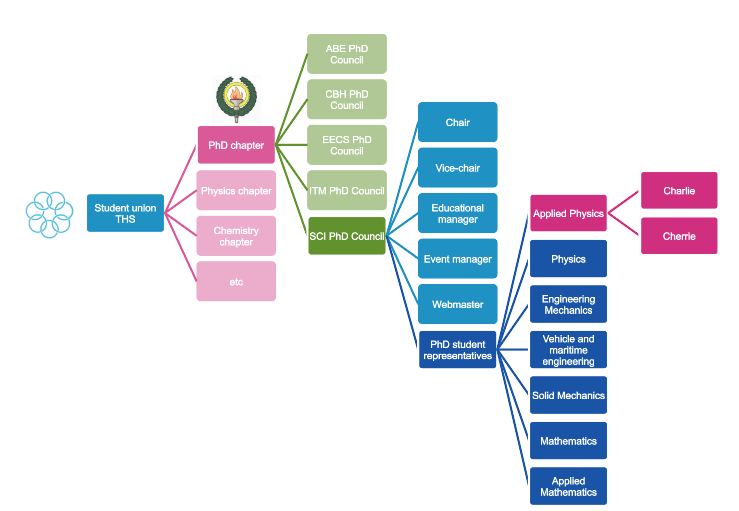
\includegraphics[width=1\linewidth]{image/Screenshot 2026-01-24 105715.png}
    \caption{Example of structure to give an idea.}
    \label{fig:placeholder}
\end{figure}

\subsection{Supervision and Conflicts}
You have the right to at least two supervisors. You are entitled to change supervisors if needed, though this is a last resort. Always try a serious discussion first; if that fails, speak with the department head or the coordinator of third-cycle education.

\subsection{Reporting channels}
Delegation orders explain how employer responsibility is distributed. If you feel unsafe, seek support from Saco-S or student union representatives. Harassment should be documented (incidents, dates, recordings if you are a participant). Reports can be made to the Vice Chancellor or Equality Ombudsman.

\subsection{Problems with your research or everyday work}
Talk to the PAD first. Psychologists are also available via KTH and can be booked anonymously: \url{https://www.kth.se/en/student/stod/halsa/studenthalsan-1.409886}.

\subsection{PhD Chapter and community}
The PhD chapter organizes parties, workshops, and pubs. Each program course has a respective organization but you also belong to the PhD chapter.
Group emails can be found at: \url{https://www.kth.se/en/tekmek/kontakt/internt-1.1223650}.

\section{Travel and Conferences}
When traveling for conferences, use \textbf{KTH-RES} (expenses/requests) and \textbf{BIG TRAVEL} (bookings).
\begin{enumerate}
    \item Create a travel request on KTH-RES with a cost estimate.
    \item Book travel through BIG TRAVEL.
    \item Use Spendcatcher or KTH-RES to track expenses during the trip.
    \item Create a travel report after the trip for reimbursement.
\end{enumerate}
Note the timing of conferences (January/February deadlines) and apply for travel scholarships during this period.

\section{Research Ethics}
\label{sec:ethics}

\subsection{Introduction to Research Ethics}

Why is research ethics important in scientific research?
\begin{itemize}
    \item \textbf{Copyright:} Protecting intellectual property and original works.
    \item \textbf{AI Ethics:} Navigating the implications of artificial intelligence in research.
    \item \textbf{Public Funding:} Research is often state-funded, requiring compliance with public standards and regulations.
\end{itemize}

Ethics addresses the fundamental question: \textit{What should we do next?}
\begin{itemize}
    \item Encourages collaborative work.
    \item Builds public support and trust.
    \item Makes science more effective and reliable.
    \item Ensures accountability.
    \item Upholds moral and social values.
\end{itemize}

\subsection{Principles of Good Research Ethics}
\label{sec:principles}

According to All European Academies (ALLEA), the core principles are:
\begin{itemize}
    \item \textbf{Reliability:} Ensuring the quality of research through rigorous methodology.
    \item \textbf{Honesty:} Presenting research in a transparent, fair, full, and unbiased way.
    \item \textbf{Respect:} For colleagues, research participants, animals, society, ecosystems, cultural heritage, and the environment.
    \item \textbf{Accountability:} Taking responsibility for the research from its inception to publication, including management, training, and mentoring.
\end{itemize}

\textit{Recommended Reading: The European Code of Conduct for Research Integrity.}

\subsection{Research Misconduct and Bad Practices}\label{sec:misconduct}

\subsubsection{Major Violations: FFP}
Fabrication, Falsification, and Plagiarism (FFP) represent the most serious violations of research integrity.

\subsubsection{Other Problematic Practices}
\begin{enumerate}
    \item Manipulating authorship.
    \item Self-plagiarism (reusing one's own work without proper citation).
    \item Citing selectively to enhance own findings or to please editors, reviewers, or colleagues.
    \item Withholding research results.
    \item Allowing funders/sponsors to jeopardize independence.
    \item Expanding the bibliography of a study unnecessarily.
    \item Accusing a researcher of misconduct or other violations in a malicious way.
    \item Misrepresenting research achievements and results.
    \item Exaggerating the importance and applicability of findings.
    \item Delaying or inappropriately hampering the work of other researchers.
    \item \textbf{Misusing seniority} to encourage violations of research integrity.
    \item \textbf{Ignoring putative violations of research integrity} by others or covering up inappropriate responses to misconduct.
    \item Establishing or supporting journals that undermine quality control (predatory journals).
\end{enumerate}

\subsection{Ethical Concerns in Research Groups}\label{sec:group_concerns}
Common issues identified in research environments include:
\begin{itemize}
    \item Resource management and use.
    \item Authorship disputes.
    \item Transparency in publication and peer review.
    \item Power dynamics and seniority.
    \item Use of AI tools in research.
    \item Personal data protection and lab safety.
    \item Reproducibility of results.
\end{itemize}

\subsection{Authorship and Publication Ethics}\label{sec:authorship}

\textbf{Why is authorship important?}
\begin{enumerate}
    \item It clarifies who bears responsibility in the event of an investigation into misconduct.
    \item Researchers are assessed for positions and funding based on their publication record.
\end{enumerate}

\subsubsection{Types of Problematic Authorship}
\begin{itemize}
    \item \textbf{Guest Authorship:} Including a senior figure (e.g., a boss) who has made no contribution.
    \item \textbf{Honorary or Gift Authorship:} Assigning authorship to someone as a favor.
    \item \textbf{Ghost Authorship:} Failing to list a significant contributor.
    \item \textbf{Authorship for Sale:} Purchasing names to be added to a manuscript.
    \item \textbf{Anonymous Authorship:} Publishing under a pseudonym or different name.
\end{itemize}

Authorship norms vary significantly across disciplines, and there are several different guidelines available.

\subsubsection{Common Authorship Principles}
The following principles are common to most authorship guidelines:
\begin{itemize}
    \item Journal editors have the prerogative to define authorship and contributorship criteria.
    \item Researchers who performed the work are responsible for identifying authors based on the journal's criteria.
    \item Every individual listed as an author should review and approve the final manuscript before publication.
    \item An author should be able to identify which co-authors are responsible for specific parts of the work.
    \item The ultimate goal is to establish accountability and transparency.
\end{itemize}

The most influential rules are the International Committee of Medical Journal Editors (ICMJE) rules, often referred to as the \textit{Vancouver rules}. KTH provides tools for authorship assessment on its website.

\subsection{Research on Human Subjects}\label{sec:human_subjects}

Guidelines such as the Nuremberg Code and the World Medical Association's Declaration of Helsinki provide the global framework for ethics in human research.

\subsection{Swedish Ethical Review Requirements}\label{sec:swedish_ethics}

In Sweden, researchers are legally responsible for applying for an ethical review for research involving human subjects (Statute 2004:405). Since January 1, 2019, applications for ethical permits are submitted to the Swedish Ethical Review Authority (\textit{Etikprövningsmyndigheten}).

\subsubsection{Areas Requiring Ethical Review}\label{sec:human_review_areas}
\begin{itemize}
    \item Processing of sensitive personal data.
    \item Physical interventions on living or deceased persons.
    \item Methods intended to influence study participants.
    \item Research on biological material taken from living or deceased persons.
\end{itemize}

You can appeal the decision from the SWEDISH ETHICAL REVIEW AUTHORITY by contacting the ETHICAL BOARD.

\newpage
\paragraph{This section}\textit{has been fully developed by Emanuele} D'Allestro.

\newpage
\section{Solid Mechanics Department}
\label{sec:solid_mechanics}

\subsection{Laboratories}
There are two main labs located at Teknikringen 8D: the \textbf{Solid Mechanics Lab} and the \textbf{Lightweight Structures Lab}. To use these facilities, you must complete a 3-hour safety course and receive an introduction from the lab managers.

\subsection{KTH Service and Logistics}
The KTH Service team at Teknikringen 8D handles various administrative and logistical tasks, including parcel deliveries. If you have incoming parcels, please use the following address:

\begin{quote}
    KTH Verksamhetsstöd\\
    Skolan för teknikvetenskap\\
    Teknikringen 8D, 100 44 Stockholm\\
    ATT: [YOUR NAME]
\end{quote}

\subsection{Academic Requirements and Courses}
As a PhD student in this department, you are required to obtain \textbf{60 credits} to defend your thesis.
\begin{itemize}
    \item \textbf{Credit Transfer:} Up to 15 credits can typically be transferred from your Master's degree. This requires submitting a credit transfer form to the Doctoral Education Support (FOA).
    \item \textbf{Mandatory Courses:} Essential courses include Research Ethics, Continuum Mechanics, and Testing Techniques.
    \item \textbf{Planning:} Note that some departmental courses are only offered every 2 or 3 years, so plan your Individual Study Plan (ISP) carefully.
    \item \textbf{Course Levels:} Courses starting with `3` (e.g., 3000-series) are doctoral level, while `2` and `1` indicate Master's and Bachelor's levels respectively.
\end{itemize}

For the credit transfer form and more information, visit: 
\url{https://intra.kth.se/en/eecs/forskarutbildning/courses/course-information-for-doctoral-students-1.813447}

\subsection{Learning Swedish}
If you wish to learn Swedish, several options are available:
\begin{itemize}
    \item \textbf{SFI (Swedish for Immigrants):} Free courses provided by the municipality.
    \item \textbf{KTH Courses:} Language courses specifically for students.
    \item \textbf{Swedish for Employees:} You can request to join these through your supervisor.
\end{itemize}

\subsection{Lunch and Social Life}
Lunch is a central social event, typically occurring between 11:30 and 13:00. Most people gather in the second-floor lounge room (where the microwaves are) around 12:00.

\subsubsection{Dining Options Near Campus}
\begin{itemize}
    \item \textbf{Syster o Bror:} A popular nearby restaurant with a buffet.
    \item \textbf{Q Building:} Offers a large lunch buffet.
    \item \textbf{Brazilia:} High-quality buffet with many vegan options.
    \item \textbf{7-Eleven:} Convenient for quick snacks (use the \textit{Karma} app for discounts).
    \item \textbf{T-Snabben:} A minimarket with a salad bar (\textit{Picadeli}).
    \item \textbf{Coffice:} Good for coffee, fika, and sandwiches.
    \item \textbf{Nymble (Student Union Building):} Offers meals with student discounts.
\end{itemize}

\textbf{Pancake Thursday:} It is a Swedish tradition to serve pea soup and pancakes on Thursdays; you will find this menu at many of the locations listed above.

\subsection{Lounge Room and Kitchen Facilities}
The lounge room is fully equipped with microwaves, refrigerators, and dishwashers. Free coffee is often available during breaks. 
\textit{Note:} Tap water in Sweden is of very high quality and perfectly safe to drink; there is no need to buy bottled water.

\input{Fluids}
\input{Lightweight Structures}


\vfill
\centering
\scriptsize © 2025 Emanuele D'Allestro. All rights reserved.
\end{document}
